\chapter{Metodología}
\label{chap:modelos}

Los fundamentos de los \textit{word embeddings} presentados en el capítulo anterior establecen el marco teórico sobre el que se construyen los algoritmos de generación de representaciones vectoriales de palabras. Este capítulo aborda en detalle los dos modelos centrales de este trabajo. En primer lugar, se describe el algoritmo clásico Word2Vec y su variante Skip-gram. A continuación se presenta QWord2Vec, la primera adaptación formal de Word2Vec al entorno cuántico. Por último, se exponen las propuestas de mejora introducidas en este Trabajo de Fin de Grado sobre el modelo cuántico original, que son la sustitución del optimizador \gls{spsa} por \gls{qn-spsa} y la inicialización guiada de los parámetros del circuito.

\section{Algoritmo Word2Vec}
\label{chap:word2vec}

Word2Vec, cuyo nombre proviene de la contracción de \textit{Word to Vector}, es un modelo de \gls{ml} que permite representar palabras como vectores de grandes dimensiones. Su principal virtud reside en que las relaciones semánticas y sintácticas entre palabras quedan codificadas como proximidad geométrica entre dichos vectores, permitiendo así capturar el significado de forma numérica y operable.

Este algoritmo fue desarrollado y publicado por Google en 2013 \cite{google_word2vec_2013}. Además, en esa misma fecha se introdujo este modelo en su motor de búsqueda. Desde entonces, el modelo ha sido ampliamente adoptado y ha dado lugar a múltiples mejoras y variantes de rendimiento.

En esta sección se explorarán la arquitectura del modelo, su función de optimización y el proceso de entrenamiento que permite generar el espacio vectorial latente en el que las palabras quedan representadas.

\subsection{Arquitectura del modelo}

Word2Vec aprende las representaciones de las palabras procesando grandes volúmenes de texto y capturando el contexto en el que aparece cada término \cite{logunova_word2vec_serokell}. Su arquitectura se fundamenta en una red neuronal superficial (\textit{shallow neural network}), que, a diferencia de las redes profundas (\textit{deep neural networks}), dispone únicamente de una capa oculta entre la capa de entrada y la de salida, tal como se ilustra en la Figura \ref{fig:comp_rnns_word2vec}. Este diseño proporciona una ventaja clave: permite entrenar el modelo de forma eficiente sobre corpus de gran tamaño manteniendo un coste computacional razonable.

\begin{figure}[h]
  \centering
  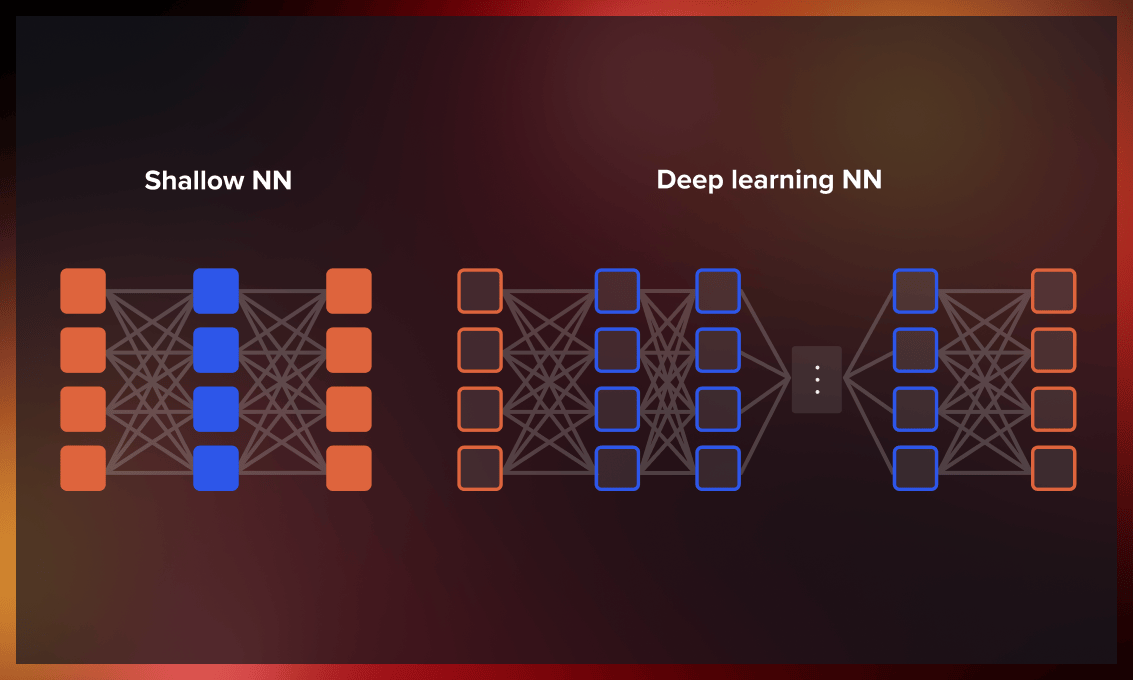
\includegraphics[width=0.8\linewidth]{imagenes/compRNNsWord2Vec.png}
  \caption{Comparativa entre una red neuronal superficial (Word2Vec) y una red neuronal profunda. Fuente: \cite{logunova_word2vec_serokell}.}
  \label{fig:comp_rnns_word2vec}
\end{figure}

El resultado del entrenamiento es la asignación de un vector de cientos de dimensiones a cada palabra del vocabulario. La posición de cada vector en ese espacio no es arbitraria: palabras empleadas en contextos similares acaban próximas entre sí, mientras que palabras semánticamente distantes se alejan geométricamente. Este hecho puede observarse en la Figura \ref{fig:representacion_word2vec}.

\begin{figure}[h]
  \centering
  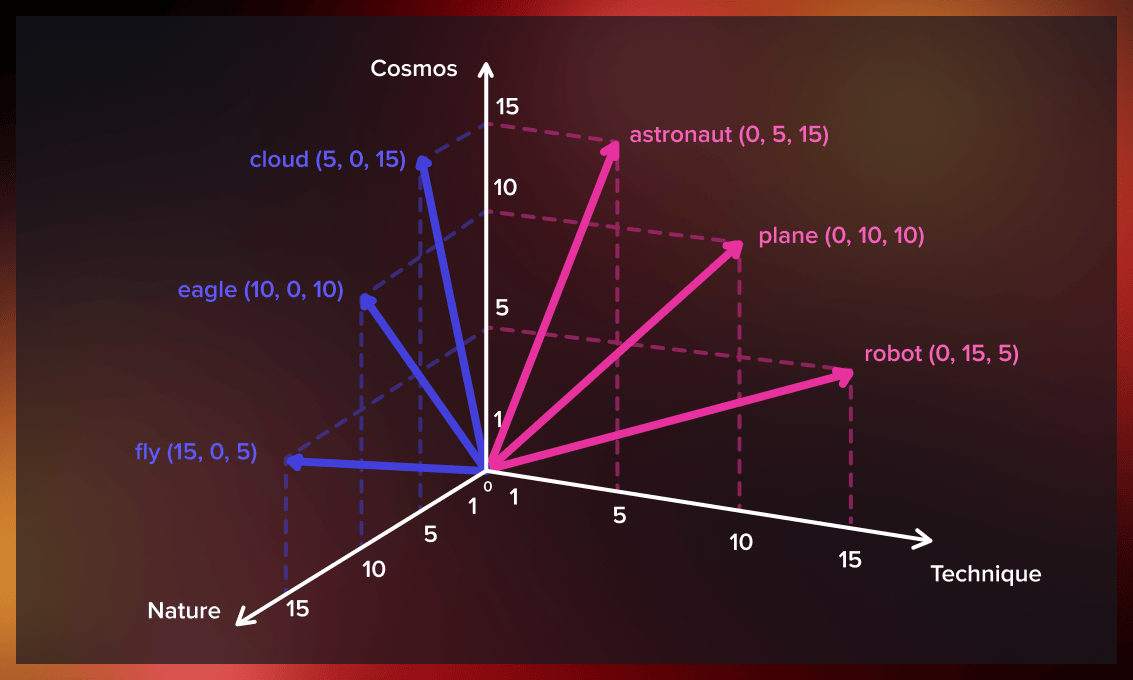
\includegraphics[width=0.8\linewidth]{imagenes/representacionWord2Vec.png}
  \caption{Representación vectorial de palabras en el espacio latente generado por Word2Vec. Fuente: \cite{logunova_word2vec_serokell}.}
  \label{fig:representacion_word2vec}
\end{figure}

Una consecuencia directa de esta estructura es que los vectores admiten operaciones algebraicas con significado semántico. El ejemplo más conocido de esta propiedad es la siguiente analogía entre género y realeza \cite{google_word2vec_2013}:

\[
  \vec{v}(\text{Rey}) - \vec{v}(\text{Hombre}) + \vec{v}(\text{Mujer}) \approx \vec{v}(\text{Reina});
\]

En esta expresión, al restar al vector de \textit{Rey} la componente que codifica la masculinidad y sumar la que codifica la feminidad, el vector resultante converge hacia la representación de \textit{Reina}. Esta propiedad es inherente a la forma natural del entrenamiento: como \textit{Rey} y \textit{Reina} comparten contextos de realeza pero difieren en los contextos de género, el modelo aprende implícitamente a separar ambas dimensiones dentro del espacio vectorial, tal y como se aprecia visualmente en la Figura \ref{fig:similitudes_palabras_word2vec}.

\begin{figure}[h]
  \centering
  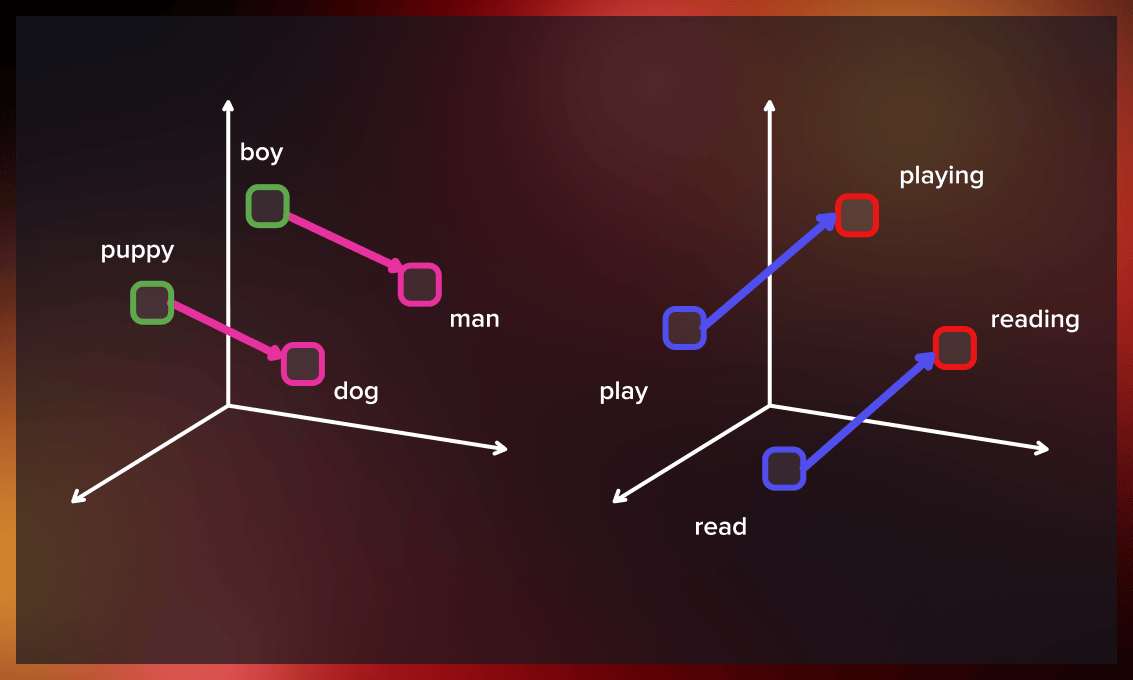
\includegraphics[width=0.8\linewidth]{imagenes/similitudesPalabrasWord2Vec.png}
  \caption{Representación geométrica de las similitudes semánticas entre palabras en el espacio vectorial de Word2Vec. Fuente: \cite{logunova_word2vec_serokell}.}
  \label{fig:similitudes_palabras_word2vec}
\end{figure}

\subsubsection{Modelos de entrenamiento: \glsentryshort{cbow} y Skip-gram}

Word2Vec ofrece dos variantes arquitectónicas para aprender los vectores de palabras \cite{google_word2vec_2013}: el modelo \textbf{\gls{cbow}} y el modelo \textbf{Skip-gram}. Ambos comparten la misma red neuronal superficial como base, pero se diferencian en el aprendizaje, en lo que se usa como entrada y en lo que se predice como salida.

En este trabajo se ha optado por implementar el modelo \textbf{Skip-gram}, ya que, como se verá en la siguiente sección, sus características lo hacen especialmente adecuado para la adaptación al entorno cuántico propuesto.

\paragraph{Continuous Bag of Words (CBOW)}

El modelo \gls{cbow} toma como entrada las palabras del contexto que rodean a una posición central y predice cuál es la palabra que debería ocupar dicha posición. En otras palabras, dadas las palabras vecinas, el modelo intenta adivinar la palabra central, como se muestra en la Figura \ref{fig:cbow_example}.

\begin{figure}[h]
  \centering
  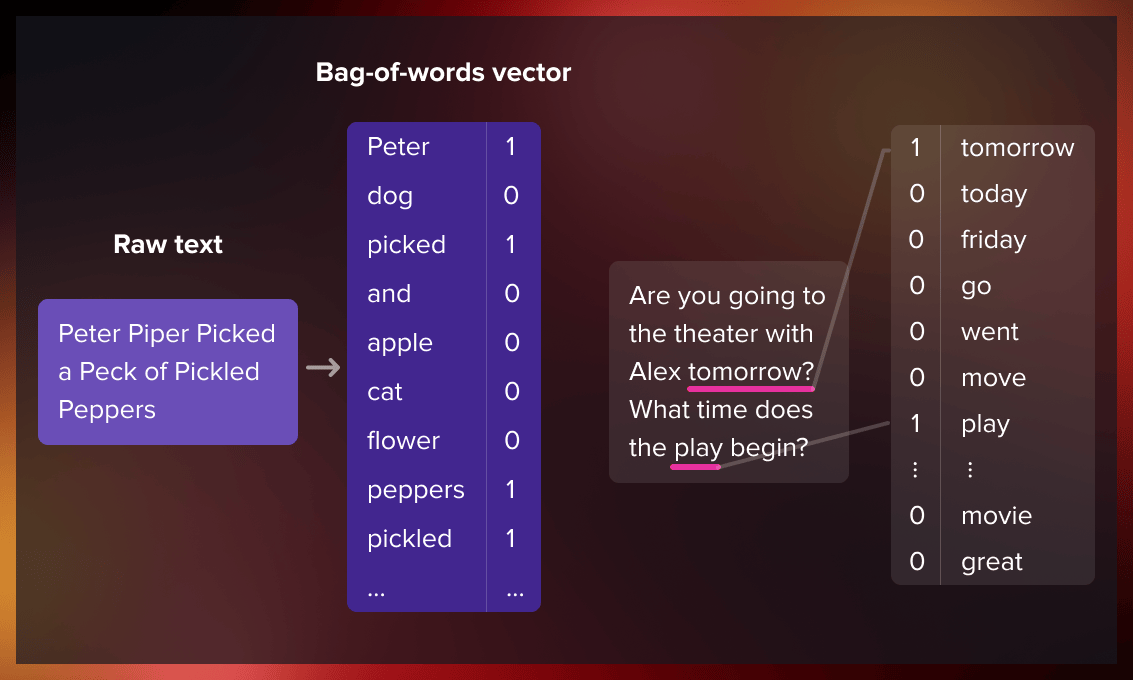
\includegraphics[width=0.8\linewidth]{imagenes/bowExample.png}
  \caption{Ejemplo del funcionamiento del modelo \gls{cbow}: a partir de las palabras de contexto circundantes se predice la palabra objetivo central. Fuente: \cite{logunova_word2vec_serokell}.}
  \label{fig:cbow_example}
\end{figure}

Este enfoque resulta eficiente cuando el corpus es grande y las palabras frecuentes tienen representaciones ricas. Sin embargo, tiende a promediar la información del contexto, lo que puede penalizar los valores semánticos de palabras menos frecuentes, generando así una pérdida de información.

\paragraph{Skip-gram}

Es un modelo diseñado para hacer lo opuesto a \gls{cbow}. En lugar de predecir la palabra central a partir del contexto que tiene en su ventana, toma una única palabra central como entrada e intenta predecir las palabras que aparecen a su alrededor.

El proceso de entrenamiento de esta red neuronal superficial funciona de la siguiente manera: dada la palabra central (la palabra de entrada), se selecciona aleatoriamente una palabra de su contexto inmediato. La red calcula cuál es la probabilidad de que cada palabra del vocabulario sea una palabra ``cercana'' a la palabra de entrada \cite{mccormick_skipgram_2016}.

Los resultados de estas probabilidades indican cuán probable es que cada término del vocabulario aparezca en las proximidades de la palabra de entrada. Por ejemplo, si la palabra de entrada proporcionada a la red ya entrenada es \textit{reino}, las probabilidades serán considerablemente mayores para palabras como \textit{España} o \textit{Inglaterra} que para términos sin relación semántica como \textit{lápiz} o \textit{mango}.

\subsubsection{Detalles del modelo básico Skip-gram}

Dado que una red neuronal no puede procesar cadenas de texto directamente, cada palabra se representa mediante un \textit{vector one-hot} (una forma de codificación sencilla aunque no la única). En este vector hay tantas componentes como palabras tiene el vocabulario (por ejemplo, 10.000), donde únicamente la posición correspondiente a la palabra de entrada vale 1 y el resto valen 0.

La capa de salida de la red produce también un vector de 10.000 componentes, donde cada valor refleja la probabilidad de que la palabra correspondiente sea una palabra cercana a la entrada. No existe función de activación en la capa oculta, pero la capa de salida aplica \textit{softmax} para normalizar las probabilidades. Esta arquitectura completa puede observarse en la Figura \ref{fig:red_skip_gram}.

\begin{figure}[h]
  \centering
  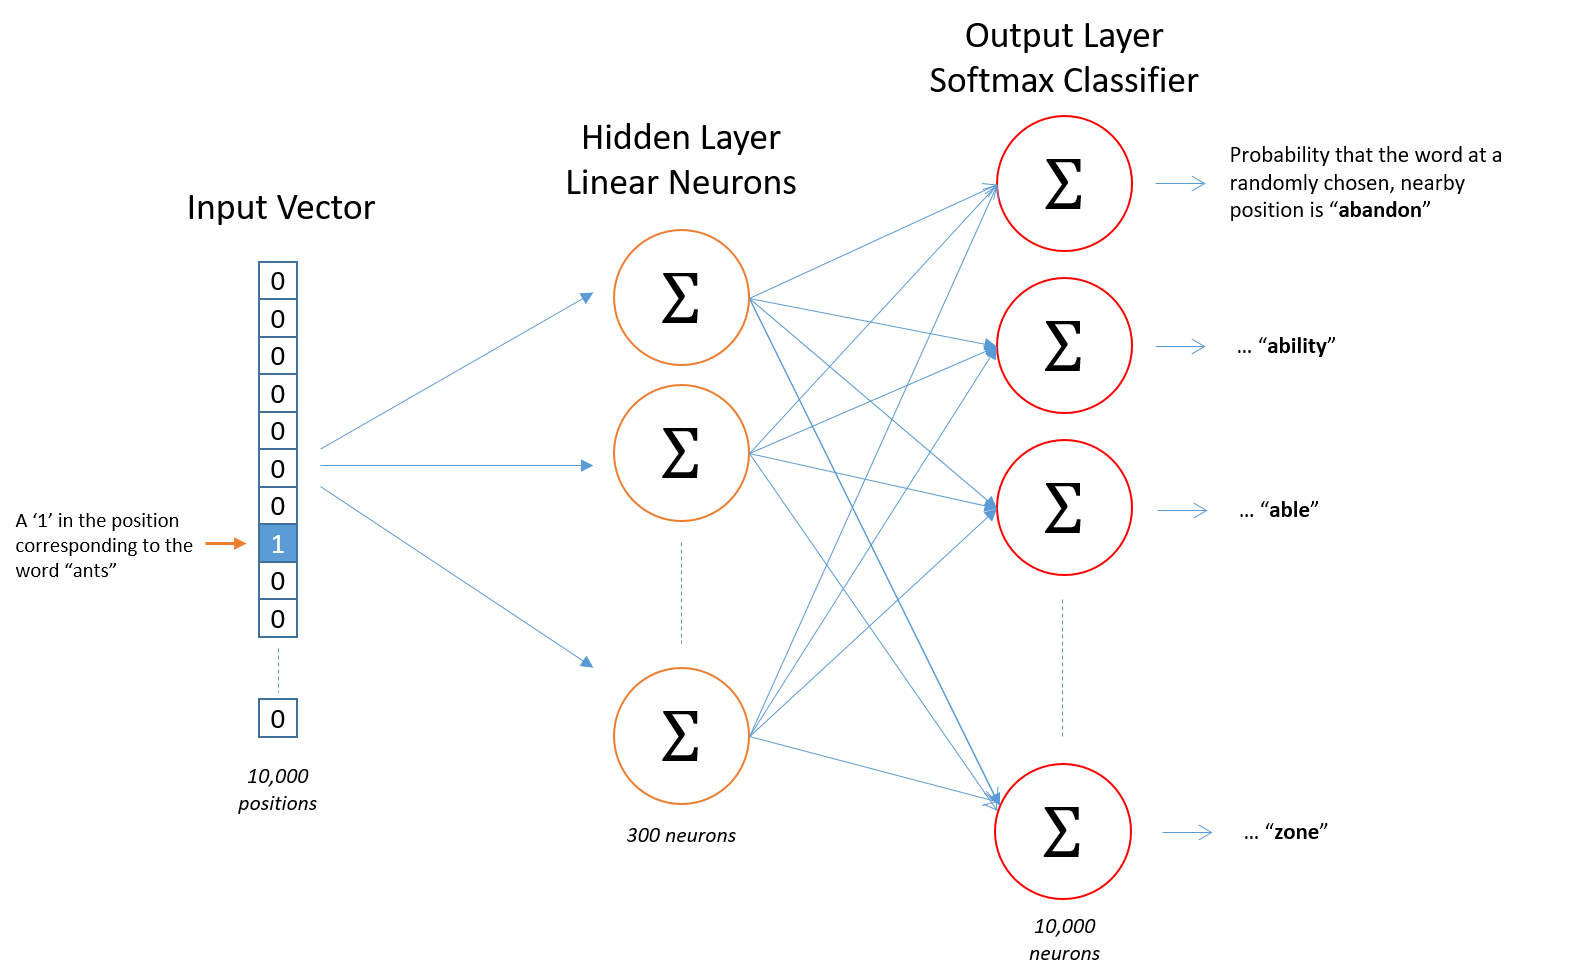
\includegraphics[width=0.9\linewidth]{imagenes/redSkipGram.png}
  \caption{Arquitectura de la red neuronal del modelo Skip-gram. Fuente: \cite{mccormick_skipgram_2016}.}
  \label{fig:red_skip_gram}
\end{figure}

Durante el entrenamiento, tanto la entrada como la salida de la red son vectores \textit{one-hot}. Por el contrario, al evaluar la red con una palabra de entrada, el vector de salida ya no es \textit{one-hot}, sino una distribución de probabilidad sobre todo el vocabulario.

A modo de ejemplo concreto, supóngase que la \textbf{capa oculta} aprende vectores de palabras de 300 dimensiones. En ese caso, los pesos de dicha capa quedan representados por una matriz de $10.000 \times 300$: una fila por cada palabra del vocabulario y una columna por cada neurona oculta. Este es precisamente el tamaño que empleó Google en el trabajo original en el que presentó Word2Vec \cite{google_word2vec_2013}.

Al final, el objetivo de este modelo es aprender la matriz de pesos de la capa oculta, cuya estructura se ilustra en la Figura \ref{fig:matriz_pesos_skip_gram}. Una vez obtenida esta matriz, la capa de salida proyecta el vector latente de vuelta al tamaño del vocabulario mediante una segunda matriz de pesos y estima la probabilidad de coocurrencia de cada palabra.

\begin{figure}[h]
  \centering
  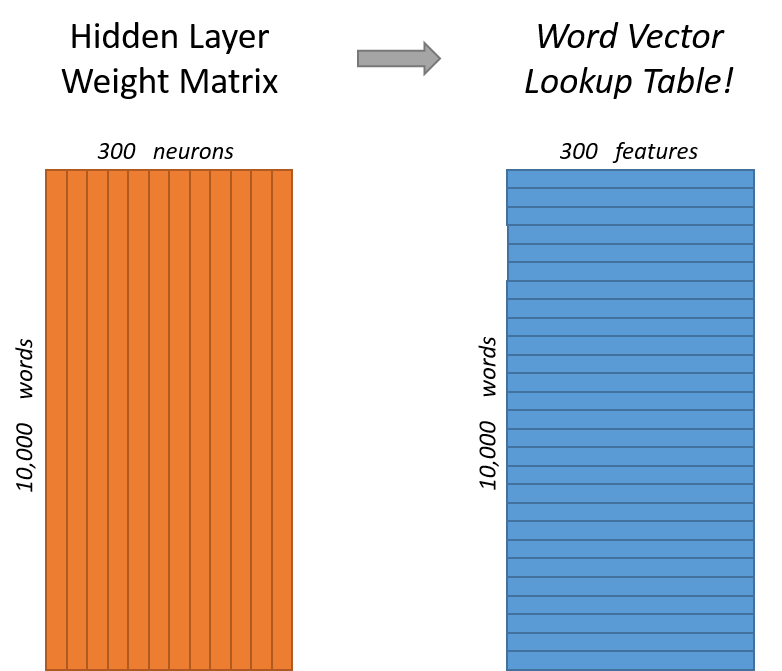
\includegraphics[width=0.6\linewidth]{imagenes/matrizPesosSkipGram.png}
  \caption{Matriz de pesos de la capa oculta del modelo Skip-gram: 10.000 filas (una por palabra del vocabulario) y 300 columnas (una por neurona oculta). Cada fila constituye el vector de representación de su palabra correspondiente. Fuente: \cite{mccormick_skipgram_2016}.}
  \label{fig:matriz_pesos_skip_gram}
\end{figure}

Llegados a este punto, uno puede preguntarse cuál es la utilidad de representar las palabras mediante vectores de todo ceros salvo una única posición con valor $1$. La respuesta reside en la eficiencia: multiplicar un vector \textit{one-hot} de $1 \times 10.000$ por la matriz de $10.000 \times 300$ selecciona de forma inmediata la fila correspondiente a la palabra de entrada sin necesidad de realizar el producto matricial completo, tal y como se muestra en la Figura \ref{fig:mult_matriz_one_hot}.

\begin{figure}[h]
  \centering
  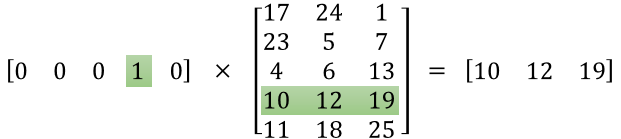
\includegraphics[width=0.7\linewidth]{imagenes/multMatrizOneHot.png}
  \caption{Multiplicación de un vector \textit{one-hot} por la matriz de pesos de la capa oculta, obteniendo directamente el vector de representación de la palabra de entrada. Fuente: \cite{mccormick_skipgram_2016}.}
  \label{fig:mult_matriz_one_hot}
\end{figure}

Con esto se concluye que la capa oculta del modelo actúa en realidad como una tabla \textit{lookup}: la salida de dicha capa es directamente el vector de representación de la palabra de entrada. Así, el vector de $1 \times 300$ resultante se pasa a la \textbf{capa de salida}, que es un clasificador de regresión \textit{softmax}.

Cada neurona de salida produce un valor entre 0 y 1 aplicando la función $\exp(x)$ sobre el producto de su vector de pesos y el vector proveniente de la capa oculta. Para que todos los valores sumen 1 y formen una distribución de probabilidad, cada resultado se divide entre la suma de los valores de las 10.000 neuronas de salida \cite{mccormick_skipgram_2016}, tal y como se aprecia en la Figura \ref{fig:ejemplo_capa_salida_skip_gram}.

\begin{figure}[h]
  \centering
  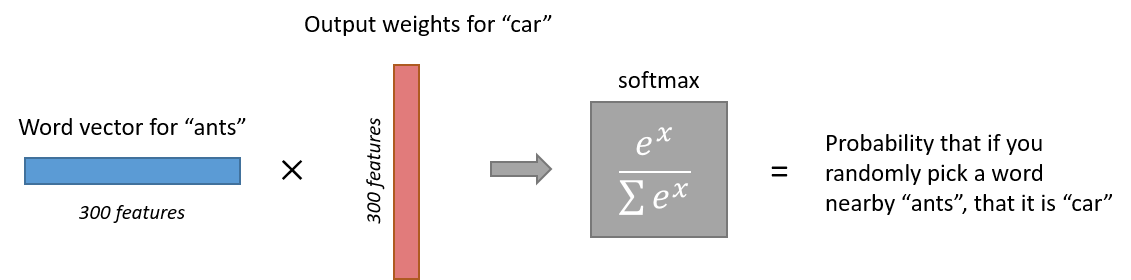
\includegraphics[width=0.9\linewidth]{imagenes/ejemploCapaSalidaSkipGram.png}
  \caption{Cálculo de la salida de la neurona correspondiente a la palabra \textit{car} en la capa \textit{softmax} del modelo Skip-gram. Fuente: \cite{mccormick_skipgram_2016}.}
  \label{fig:ejemplo_capa_salida_skip_gram}
\end{figure}

\subsubsection{Mejoras aplicadas al modelo básico Skip-gram}

Retomando el ejemplo anterior de Skip-gram, con 300 dimensiones y un vocabulario de 10.000 palabras, la red neuronal dispone de dos matrices de pesos: una correspondiente a la capa oculta y otra a la capa de salida. Cada una de ellas contiene un total de $300 \times 10.000 = 3$ millones de parámetros. Para ajustar correctamente este volumen de parámetros y evitar al mismo tiempo el sobreajuste se debe disponer de conjuntos de datos de entrenamiento de gran tamaño, lo que convierte el entrenamiento del modelo básico en un proceso computacionalmente costoso.

Para abordar este problema, Google publicó un segundo artículo \cite{mikolov_skipgram_phrases_2013} en el que se proponían dos innovaciones clave sobre el modelo básico:

\begin{itemize}
  \item \textbf{Submuestreo de palabras frecuentes}: se reduce la frecuencia con la que las palabras muy comunes participan en el entrenamiento, disminuyendo así el número total de ejemplos procesados. Para ello, cada palabra $w_i$ del corpus se descarta durante el entrenamiento con una probabilidad dada por $P(w_i) = 1 - \sqrt{t / f(w_i)}$, donde $f(w_i)$ es la frecuencia de la palabra y $t$ es un umbral de tolerancia típico (por ejemplo, $10^{-5}$).
  \item \textbf{\textit{Negative Sampling}}: se sustituye la función de optimización original (descenso del gradiente) por una alternativa más eficiente que, en lugar de actualizar todos los pesos de la red en cada iteración, únicamente modifica un subconjunto reducido de ellos.
\end{itemize}

Estas dos mejoras demostraron que, lejos de comprometer la calidad del modelo, se conseguía una reducción del coste computacional y una mayor calidad de los vectores de palabras resultantes. Dado que en la implementación práctica de este trabajo se ha empleado el \textit{Negative Sampling} como función de optimización, su funcionamiento se describe en detalle en la sección siguiente.

\subsection{Función de optimización}

Para comprender la mejora que introduce el \textit{Negative Sampling} es necesario partir de la formulación matemática original del modelo básico de Skip-gram y, a partir de ella, entender qué limitaciones motivan la adopción de esta nueva función de optimización \cite{tsang_skipgram_review_medium}.

El objetivo principal de Skip-gram es maximizar la probabilidad logarítmica promedio sobre todo el corpus de entrenamiento, lo que queda expresado mediante la siguiente fórmula:

\[
  \frac{1}{T} \sum_{t=1}^{T} \sum_{\substack{-c \leq j \leq c \\ j \neq 0}} \log p(w_{t+j} \mid w_t),
\]

donde:

\begin{itemize}
  \item $c$ es el tamaño de la ventana de contexto. Valores más altos de $c$ generan más ejemplos de entrenamiento y, por tanto, ofrecen mayor precisión, aunque a costa de un tiempo de entrenamiento superior.
  \item $T$ es el número total de palabras del corpus de entrenamiento.
  \item $w_t$ es la palabra de entrenamiento en la posición $t$.
\end{itemize}

La probabilidad condicional $p(w_{t+j} \mid w_t)$ del modelo básico de Skip-gram se define mediante la función \textit{softmax} de la siguiente forma \cite{tsang_skipgram_review_medium}:

\[
  p(w_O \mid w_I) = \frac{\exp\!\left({v'_{w_O}}^{\top} v_{w_I}\right)}{\displaystyle\sum_{w=1}^{W} \exp\!\left({v'_{w}}^{\top} v_{w_I}\right)};
\]

donde $v_w$ y $v'_w$ son, respectivamente, los vectores de representación de \textit{entrada} y de \textit{salida} de la palabra $w$, y $W$ es el número total de palabras del vocabulario.

Esta formulación presenta un problema de escalabilidad: el coste de calcular $p(w_O \mid w_I)$ es proporcional a $W$, cuyo valor suele ser muy elevado (entre $10^5$ y $10^7$ términos). Esto implica que, en el denominador del \textit{softmax}, es necesario acumular los valores exponenciales de todas las palabras del vocabulario en cada paso de entrenamiento, lo que hace que el proceso resulte prohibitivamente lento cuando el vocabulario es de gran escala. Es precisamente este coste el que motiva la introducción del \textit{Negative Sampling} como función de optimización alternativa.

Esta nueva función de optimización persigue maximizar la similitud entre las palabras que aparecen en el mismo contexto y minimizarla cuando proceden de contextos distintos. Sin embargo, en lugar de aplicar esa minimización sobre todas las palabras del corpus, selecciona aleatoriamente $k$ palabras, denominadas \textit{muestras negativas}, y las emplea para optimizar la función objetivo \cite{karimi_negative_sampling_baeldung_2025}. La expresión de dicha función es la siguiente:

\[
  \log \sigma\!\left({v'_{w_O}}^{\!\top} v_{w_I}\right)
  + \sum_{i=1}^{k} \mathbb{E}_{w_i \sim P_n(w)}\!\left[\log \sigma\!\left(-{v'_{w_i}}^{\!\top} v_{w_I}\right)\right],
\]

donde $\sigma$ es la función sigmoide y $P_n(w)$ es la distribución de ruido a partir de la cual se extraen las muestras negativas. Esta distribución se calcula como la distribución unigrama de las palabras elevada a la potencia $\frac{3}{4}$, exponente elegido empíricamente en el trabajo original donde se introduce este algoritmo \cite{mikolov_skipgram_phrases_2013}:

\[
  P_n(w) = \frac{U(w)^{\frac{3}{4}}}{Z},
\]

siendo $U(w)$ la frecuencia de aparición de la palabra $w$ en el corpus y $Z$ la constante de normalización que garantiza que la distribución sume 1.

Maximizar esta expresión conlleva maximizar el producto escalar en su primer término y minimizarlo en el segundo. Dicho de otra manera, las palabras que aparecen en el mismo contexto se ven forzadas a adquirir representaciones vectoriales más similares entre sí, mientras que las que pertenecen a contextos distintos se ven forzadas a tener vectores menos similares \cite{karimi_negative_sampling_baeldung_2025}.

En cuanto a la elección del hiperparámetro $k$, el segundo artículo de Google sobre Word2Vec \cite{mikolov_skipgram_phrases_2013} indica que un valor en el rango de 5 a 20 es adecuado para corpus de entrenamiento de tamaño reducido, mientras que para corpus de gran escala se recomienda utilizar valores de entre 2 y 5.

\section{Algoritmo QWord2Vec}
\label{chap:qword2vec}

En la sección anterior se describió en detalle el algoritmo Word2Vec clásico y su variante Skip-gram, que emplea redes neuronales superficiales para aprender representaciones vectoriales de palabras a partir de grandes corpus de texto. En esta sección se presenta \textit{QWord2Vec}, una adaptación cuántica de dicho modelo propuesta por Ohno \cite{ohno_qword2vec_2025}, cuyo objetivo es explorar si el uso de circuitos cuánticos paramétricos puede ofrecer ventajas en la calidad de las representaciones vectoriales de palabras.

En esta sección se explorarán la arquitectura del circuito cuántico y la función de coste empleada para su optimización. La estrategia de optimización empleada en este trabajo se describe en la Sección~\ref{sec:propuestas_mejora}, como parte de las propuestas de mejora introducidas.

\subsection{Adaptación del algoritmo al entorno cuántico}

El circuito cuántico de \textit{QWord2Vec} sigue una estructura análoga a la de Word2Vec, compuesta por una fase de \textbf{codificación} y otra de \textbf{decodificación}. Está formado por puertas de rotación de Pauli (unitarias parametrizadas) y puertas de Pauli-X controladas (CNOT) para introducir entrelazamiento, organizadas en una estructura de capas con profundidad ajustable. Esta configuración permite procesar un estado cuántico de entrada correspondiente a la codificación \textit{one-hot} de una palabra y proyectarlo hacia un estado de salida que representa su contexto \cite{ohno_qword2vec_2025}.

\subsection{Diseño del Circuito Cuántico Parametrizado}

Como se indicó con anterioridad, la arquitectura de \textit{QWord2Vec} mantiene una estructura análoga a la del algoritmo clásico, dividiéndose en una fase de codificación y otra de decodificación. Esta similitud estructural se ilustra en la Figura \ref{fig:resumen_circuito_qword2vec}.

\begin{figure}[h]
  \centering
  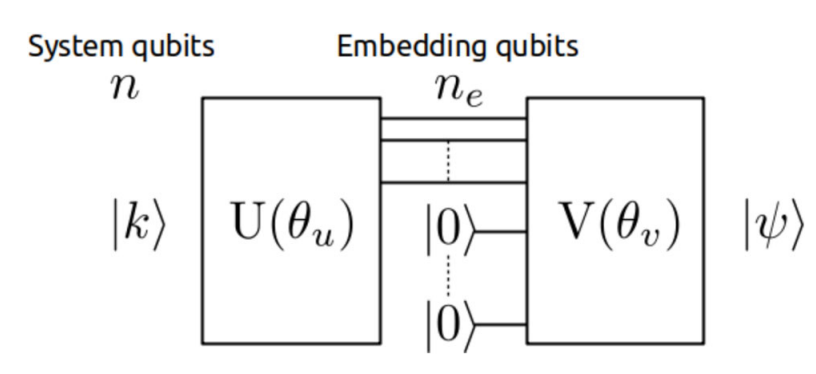
\includegraphics[width=0.9\linewidth]{imagenes/resumenCircuitoQWord2Vec.png}
  \caption{Estructura de QWord2Vec. Fuente: \cite{ohno_qword2vec_2025}.}
  \label{fig:resumen_circuito_qword2vec}
\end{figure}

En la imagen anterior, se aprecia como hay dos matrices parametrizadas, $U(\theta_u)$ y $V(\theta_v)$, junto a una matriz unitaria de entrelazamiento $U(_\text{enta})$. En este sistema, $n$ denota el número total de qubits, mientras que $n_e$ indica el número de qubits destinados específicamente a la representación de los \textit{embeddings}, debiendo cumplirse la restricción $1 \leq n_e \leq n$.

La entrada al circuito viene dada por el estado cuántico $\ket{k}$, el cual representa a una palabra codificada mediante un vector \textit{one-hot} en Word2Vec donde $0 \leq k \leq 2^n - 1$. A partir de este estado inicial, el sistema evoluciona hacia un estado de salida $\ket{\psi}$. Parecido al mapeo directo que realiza Word2Vec, el mapeo que hay entre $\ket{k}$ y $\ket{\psi}$ lo realizan los bloques $U$ y $V$.

Los estados cuánticos de salida resultantes codifican la información correspondiente al contexto de la palabra de entrada, cuya extracción se lleva a cabo realizando mediciones en la base computacional (observable Pauli $Z$).

Los modelos $U(\theta_u)$ y $V(\theta_v)$ utilizan las matrices unitarias parametrizadas y las matrices unitarias ($U_\text{enta}$) para proporcionar el entrelazamiento cuántico de la siguiente manera:

\[
  U(\theta) = \prod_{l=1}^{L}
  U_{\text{enta}}\,
  R_Z\!\left(\theta_z^{L-l+1}\right)^{\otimes n}
  R_Y\!\left(\theta_y^{L-l+1}\right)^{\otimes n}
  R_X\!\left(\theta_x^{L-l+1}\right)^{\otimes n};
\]

donde $L$ representa la longitud del circuito cuántico. Por simplicidad, se asumirá que tanto $U(\theta_u)$ y $V(\theta_v)$ poseen la misma profundidad, a menos que se indique explícitamente lo contrario.

Para implementar $U_\text{enta}$, se ha usado puertas controladas Pauli $X$ (CNOT) siguiendo una configuración de circuito por bloques \cite{sim2019expressibility}. Esta disposición favorece notablemente la expresividad del circuito y maximiza su capacidad para generar entrelazamiento. La Figura \ref{fig:qword2vec_circuit} muestra visualmente la estructura del circuito resultante al combinar las rotaciones de Pauli con el bloque de entrelazamiento descrito.

\begin{figure}[h]
  \centering
  
\includegraphics[width=1.0\linewidth]{imagenes/qword2vec_circuit.png}
  \caption{Circuito cuántico parametrizado de QWord2Vec con puertas de rotación de Pauli ($R_X$, $R_Y$, $R_Z$) y entrelazamiento con configuración por bloques mediante puertas CNOT.}
  \label{fig:qword2vec_circuit}
\end{figure}

El uso combinado de las tres puertas de rotación ($R_X, R_Y, R_Z$) permite que los estados cuánticos que representan a las distintas palabras alcancen una mayor dispersión en el espacio de Hilbert, superando las limitaciones de representatividad que se obtendrían empleando una sola matriz de rotación. Este fenómeno se observa en la Figura \ref{fig:esferas_bloch_rotaciones_pauli}.

\begin{figure}[h]
  \centering
  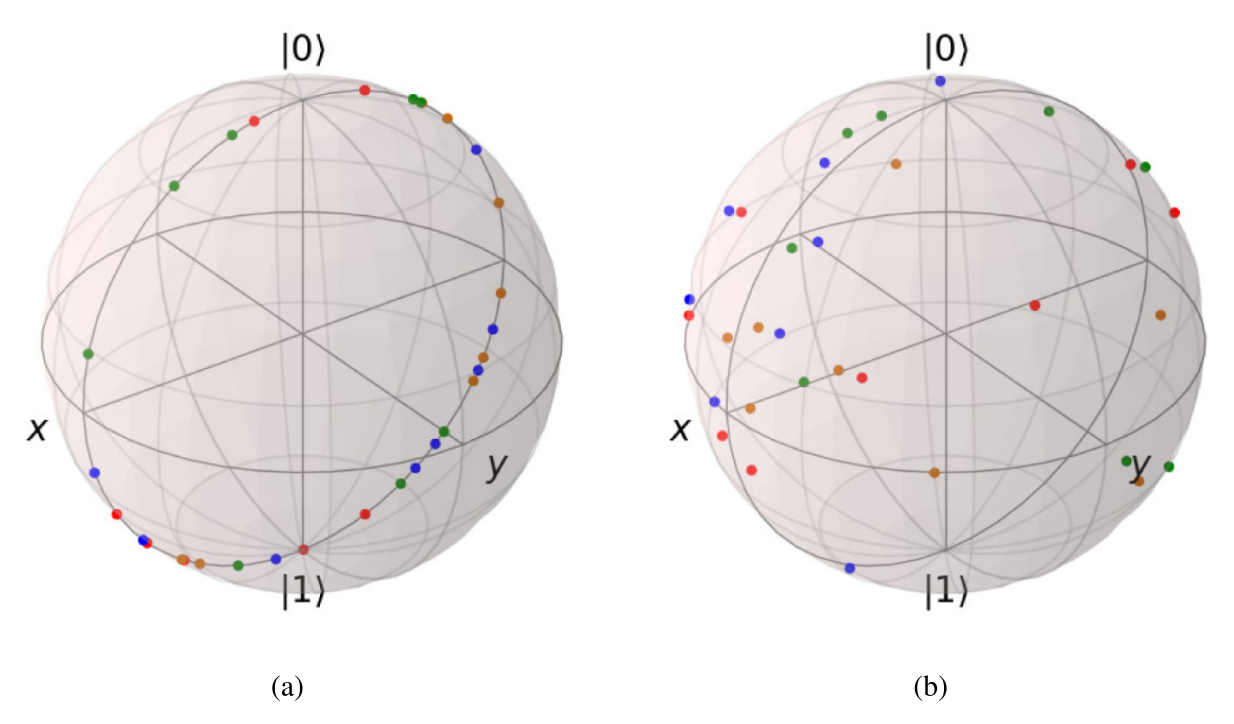
\includegraphics[width=0.9\linewidth]{imagenes/esferaBlochRotacionesPauli.png}
  \caption{Representación de las palabras sobre la esfera de Bloch según las puertas de rotación empleadas en $U(\theta_u)$: (a) usando únicamente $R_Y$, y (b) usando $R_X$, $R_Y$ y $R_Z$ combinadas. Los puntos coloreados corresponden a las palabras y el número total de puntos es 32. El uso de las tres puertas de rotación de Pauli permite una mayor dispersión de las representaciones a lo largo del espacio de Hilbert. Fuente: \cite{ohno_qword2vec_2025}.}
  \label{fig:esferas_bloch_rotaciones_pauli}
\end{figure}

\subsubsection{Estimación de la longitud del circuito}

Con el fin de acotar el espacio de búsqueda durante el ajuste de hiperparámetros, se emplea la fórmula heurística propuesta en \cite{ohno_qword2vec_2025} para estimar la profundidad $L$ del circuito cuántico:

\[
  L = \left\lceil \frac{\# \mathit{data}}{3(n + n_e)A_{th}} p(n, n_e) \right\rceil;
\]

donde los términos que intervienen en la expresión son:

\begin{itemize}
  \item $\#\mathit{data}$: número de pares de entrenamiento disponibles.
  \item $n$: número total de qubits del sistema.
  \item $n_e$: número de qubits de embeddings.
  \item $A_{th}$: umbral de tolerancia determinado de forma empírica.
  \item $p(n, n_e) \in [0, 0.5)$: probabilidad de error en función de $n$ y $n_e$.
\end{itemize}

La expresión determina la profundidad mínima necesaria para que la cantidad promedio de datos por parámetro no supere el umbral $A_{th}$. Dado que cada capa aporta $3(n + n_e)$ parámetros entrenables (un parámetro entrenable por cada matriz de rotación de Pauli), la fórmula divide la carga total de entrenamiento entre dicha capacidad ponderada por el umbral. La función techo $\lceil \cdot \rceil$ garantiza que $L$ tome un valor entero.

La probabilidad de error $p(n, n_e)$ se obtiene a partir de la siguiente inecuación, la cual relaciona la probabilidad de error entre $n$ y $n_e$:

\[
  n_e \geq (1 - H(p)) \cdot 2^n;
\]

donde $H(p)$ es la función de entropía binaria, representada en la Figura \ref{fig:entropia_binaria}.

\begin{figure}[h]
  \centering
  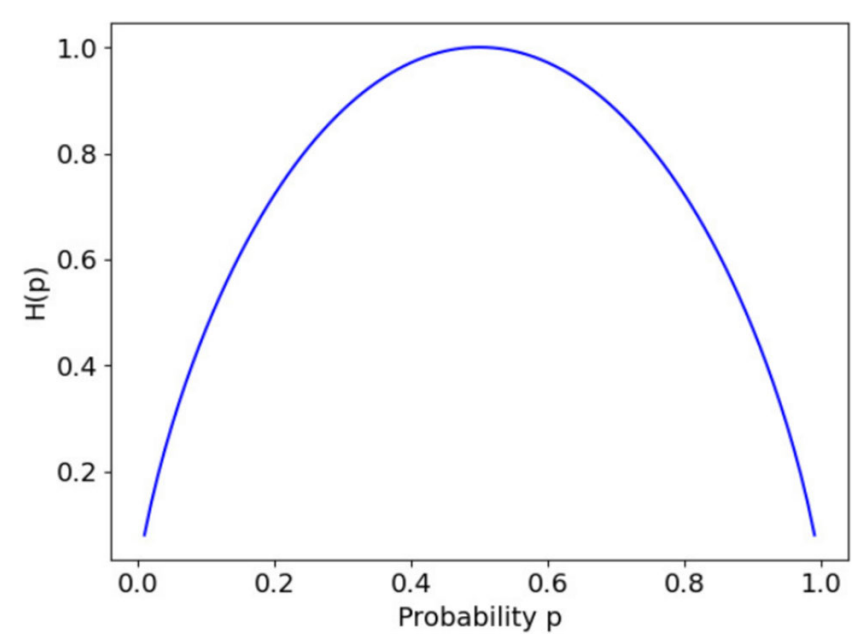
\includegraphics[width=0.6\linewidth]{imagenes/entropiaBinaria.png}
  \caption{Entropía binaria $H(p)$, donde $p$ denota la probabilidad de error empleada en este estudio. Fuente: \cite{ohno_qword2vec_2025}.}
  \label{fig:entropia_binaria}
\end{figure}

\subsection{Definición de la función de evaluación y pérdida usadas}

A continuación se procederá a explicar cuáles han sido las funciones de evaluación y de pérdidas que han sido utilizadas para entrenar a este modelo, ya que difieren completamente de la aproximación clásica seguida.

\subsubsection{Evaluación de los datos de embeddings}

Para evaluar la calidad de los \textit{embeddings} generados por QWord2Vec se emplea el coeficiente de correlación de Pearson, calculado a partir de las distancias entre los vectores producidos por ambos modelos: Word2Vec y QWord2Vec.

Una vez completado el entrenamiento, se realiza una medición sobre los qubits destinados a los \textit{embeddings}, obteniendo así los vectores clásicos correspondientes a cada palabra. A partir de estos vectores se construye un \textit{vector distancia} cuyas componentes son las distancias euclídeas entre los vectores de \textit{embeddings} de todas las palabras del vocabulario. Este proceso se aplica tanto al modelo clásico como al cuántico, tomando el vector distancia de Word2Vec como referencia de comparación (\textit{ground truth}).

El motivo por el que no se utiliza únicamente la entropía cruzada como métrica de evaluación es que los circuitos cuánticos con un elevado número de parámetros tienden a reducir su valor. Por ello, se añade el coeficiente de correlación de Pearson sobre los vectores distancia, puesto que constituye una métrica más adecuada y robusta para valorar la capacidad del modelo. En la siguiente subsección se describe en detalle la función de pérdida empleada durante el entrenamiento del circuito.

\subsubsection{Función de pérdida}

La función de pérdida diseñada para el modelo combina dos métricas. En primer lugar, emplea la \textit{entropía cruzada}, una métrica que evalúa el grado de acierto de las predicciones de un modelo frente a la realidad. Su propósito es penalizar los errores, de modo que cuanto más se alejen las predicciones de la etiqueta real, mayor será el valor de la pérdida. En el contexto de QWord2Vec, la entropía cruzada cuantifica el error entre la distribución de probabilidad estimada por el circuito cuántico $P(\theta)$ y la distribución objetivo $Y$ que dicta el contexto correcto de cada palabra central. Matemáticamente, se expresa de la siguiente manera:

\[
  \mathcal{L}_{\text{CE}} = - \sum_{i=1}^{N} Y_i \log P_i(\theta),
\]

donde $N = 2^n$ es la dimensión del espacio de Hilbert (tamaño del vocabulario). El vector $Y$ de etiquetas se obtiene de la siguiente forma: Dada una palabra objetivo del corpus, se asigna un valor de $0.5$ a las dos palabras inmediatamente adyacentes a la palabra de referencia y se establecen a cero el resto de las posiciones del vector de etiquetas de tamaño $N = 2^n$. De este modo, el vector resultante suma $1$ y representa una distribución de probabilidad uniforme sobre los dos contextos posibles de cada palabra objetivo.

A este componente clásico se añade también un segundo término basado en el coeficiente de correlación de Pearson, el cual actúa como mecanismo para garantizar la fidelidad de las representaciones espaciales en el espacio de Hilbert frente a la estructura geométrica euclídea del modelo clásico de referencia. De este modo, la función de pérdida global se expresa como:

\[
  \mathcal{L} = \mathcal{L}_{\text{CE}} - C \cdot \rho(D_{\text{QW2V}}, D_{\text{W2V}}),
\]

donde $C > 0$ es un parámetro de balanceo y $\rho(D_{\text{QW2V}}, D_{\text{W2V}})$ denota el coeficiente de correlación de Pearson, calculado como:

\[
  \rho(D_{\text{QW2V}}, D_{\text{W2V}}) = \frac{\operatorname{Cov}(D_{\text{QW2V}}, D_{\text{W2V}})}{\sigma(D_{\text{QW2V}}) \sigma(D_{\text{W2V}})},
\]

siendo $D_{\text{QW2V}}$ el vector de distancias euclídeas entre las representaciones vectoriales generadas por QWord2Vec para todas las palabras del vocabulario, $D_{\text{W2V}}$ el vector homólogo de distancias euclídeas de Word2Vec, $\operatorname{Cov}$ la covarianza y $\sigma$ la desviación estándar de sus respectivos vectores.


\section{Propuestas de mejora sobre QWord2Vec}
\label{sec:propuestas_mejora}

Del análisis del modelo QWord2Vec original propuesto por Ohno \cite{ohno_qword2vec_2025} se desprenden varias limitaciones que condicionan su rendimiento. La más relevante se encuentra en el proceso de optimización: el entrenamiento original utiliza el optimizador \gls{spsa} y requiere un número muy elevado de iteraciones (hasta $20\,000$) para alcanzar la convergencia, lo que, unido al coste exponencial de la simulación clásica de circuitos, encarece de forma notable el entrenamiento. A esta dificultad se suma la fuerte dependencia del resultado respecto a la inicialización de los parámetros del circuito y a la propia naturaleza estocástica del optimizador, factores que dificultan una convergencia estable y reproducible.

Partiendo de esta base, el presente Trabajo de Fin de Grado propone dos vías de mejora orientadas a mitigar estos problemas. En primer lugar, se sustituye el optimizador \gls{spsa} original por \gls{qn-spsa} (\textit{Quantum Natural Simultaneous Perturbation Stochastic Approximation}), que incorpora información sobre la geometría del espacio de estados cuánticos a través del tensor de Fubini-Study. En segundo lugar, se introduce una estrategia de inicialización informada de los parámetros (\textit{educated guess}) que reduce la dependencia respecto a la aleatoriedad inicial.


\subsection{Sustitución del optimizador: de SPSA a QN-SPSA}

El artículo de referencia \cite{ohno_qword2vec_2025} emplea el optimizador \gls{spsa} estándar para el entrenamiento de QWord2Vec. En este trabajo se propone sustituirlo por \gls{qn-spsa}, desarrollado por Gacon et al. \cite{gacon_qnspsa_2021}. En cada paso de optimización se requiere únicamente 2 ejecuciones del circuito cuántico para estimar el gradiente y otras 4 para aproximar el tensor métrico de Fubini-Study, con un coste independiente del número de parámetros del circuito. Esta capacidad de escalado lo convierte en un candidato especialmente adecuado para tareas de optimización en dispositivos \gls{nisq}.

Para comprender el funcionamiento de \gls{qn-spsa}, a continuación se describen los algoritmos fundamentales en los que se basa \cite{duan_qnspsa_pennylane_2022}.

\subsubsection{Funcionamiento del algoritmo}

Los optimizadores empleados en \glspl{cvc} operan bajo el mismo principio que los utilizados en \gls{ml} clásico. En cada iteración estiman el gradiente de la función de coste y, a partir de este, actualizan los parámetros del modelo con el objetivo de minimizar dicha función.

El punto de partida es el algoritmo \textit{Gradient Descent} (GD, o descenso de gradiente), cuya regla de actualización de parámetros es:

\[
  \mathbf{x}^{(t+1)} = \mathbf{x}^{(t)} - \eta \nabla f(\mathbf{x}^{(t)});
\]

donde $f$ es la función de pérdida, $\mathbf{x}$ el vector de parámetros, $\eta$ la tasa de aprendizaje y el superíndice $t$ la iteración actual. El gradiente $\nabla f$ se calcula dimensión a dimensión, lo que implica $\mathcal{O}(d)$ mediciones cuánticas, siendo $d$ el número de parámetros entrenables. Dado el elevado coste de las mediciones en un circuito cuántico, el \gls{gd} resulta inviable para circuitos con un número alto de parámetros o un gran número de iteraciones para la optimización.

Para resolver este problema de escalado surgió el optimizador \gls{spsa} (\textit{Simultaneous Perturbation Stochastic Approximation}) \cite{wikipedia_spsa_2026}. En lugar de calcular el gradiente componente a componente, \gls{spsa} selecciona una dirección aleatoria $\mathbf{h} \in U(\{-1, 1\}^d)$, donde $U(\{-1, 1\}^d)$ es una distribución uniforme discreta de $d$ dimensiones, y estima el gradiente proyectado mediante una aproximación de diferencias finitas con perturbación $\epsilon$:

\[
  \nabla_{\mathbf{h}} f(\mathbf{x}) \equiv \mathbf{h} \cdot \nabla f(\mathbf{x}) \simeq \frac{1}{2\epsilon} \bigl(f(\mathbf{x} + \epsilon \mathbf{h}) - f(\mathbf{x} - \epsilon \mathbf{h})\bigr).
\]

A partir de esta expresión se construye el estimador estocástico del gradiente:

\[
  \widehat{\nabla} f(\mathbf{x}, \mathbf{h})_{\text{SPSA}} = \nabla_{\mathbf{h}} f(\mathbf{x})\, \mathbf{h},
\]

con lo que la regla de actualización de parámetros queda:

\[
  \mathbf{x}^{(t+1)} = \mathbf{x}^{(t)} - \eta\, \widehat{\nabla} f(\mathbf{x}^{(t)}, \mathbf{h}^{(t)})_{\text{SPSA}},
\]

donde $\mathbf{h}^{(t)}$ se muestrea en cada iteración. Al tratarse de una aproximación estocástica, el gradiente estimado no es exacto. No obstante, se ha demostrado que el algoritmo converge de forma efectiva cuando se realizan suficientes iteraciones de optimización.

Sin embargo, \gls{spsa} hereda del \gls{gd} el problema de operar en el espacio euclídeo de los parámetros, lo que hace que el resultado de la optimización dependa de la parametrización elegida. Para eliminar esta dependencia, Amari (1998) propuso el algoritmo clásico \textit{Natural Gradient Descent}, que reformula el problema de optimización en términos de distribuciones de probabilidad sobre las posibles salidas del modelo. De este modo, cada paso de optimización resulta invariante frente a reparametrizaciones, ya que se realiza en el espacio de distribuciones en lugar del espacio de parámetros. Su regla de actualización incorpora la matriz de información de Fisher $F$ como tensor métrico:

\[
  \mathbf{x}^{(t+1)} = \mathbf{x}^{(t)} - \eta F^{-1} \nabla f(\mathbf{x}^{(t)}).
\]

Esta matriz actúa como un tensor métrico que transforma los pasos de descenso realizados en el espacio euclídeo de los parámetros en pasos de descenso en el espacio de distribuciones de probabilidad.

La versión cuántica de este algoritmo, el algoritmo \textit{Quantum Natural Gradient Descent} (QNG) \cite{stokes_qng_2020}, traslada este mismo principio al espacio de estados cuánticos. En dicho espacio, el tensor métrico invariante es el \textbf{tensor de Fubini-Study} $\mathbf{g}$, de dimensiones $d \times d$, definido como:

\[
  g_{ij}(\mathbf{x}) = -\frac{1}{2} \frac{\partial}{\partial \mathbf{x}_i} \frac{\partial}{\partial \mathbf{x}_j} F(\mathbf{x}', \mathbf{x}) \bigg|_{\mathbf{x}'=\mathbf{x}},
\]

donde $F(\mathbf{x}', \mathbf{x}) = \left| \braket{\phi(\mathbf{x}')}{\phi(\mathbf{x})} \right|^2$ y $\phi(\mathbf{x})$ es el circuito ansatz parametrizado con entrada $\mathbf{x}$. La regla de actualización de \gls{qng} es:

\[
  \mathbf{x}^{(t+1)} = \mathbf{x}^{(t)} - \eta\, \mathbf{g}^{-1}(\mathbf{x}^{(t)}) \nabla f(\mathbf{x}^{(t)}).
\]

El uso del tensor $\mathbf{g}$ permite una convergencia más rápida y hacia mejores mínimos que el \gls{gd}. No obstante, su cálculo requiere un gran número de mediciones cuánticas, lo que lo hace igualmente inescalable para circuitos de gran tamaño y con gran número de iteraciones para optimizarlos.

\gls{qn-spsa} surge precisamente como solución a esta limitación, combinando las ventajas de \gls{spsa} y \gls{qng}. Estima de forma estocástica tanto el gradiente como el tensor de Fubini-Study, manteniendo un coste constante independiente de $d$. El gradiente se estima con el mismo procedimiento que en \gls{spsa}, mientras que el tensor se aproxima mediante un estimador de segundo orden con dos perturbaciones estocásticas adicionales:

\[
  \widehat{\mathbf{g}}(\mathbf{x}, \mathbf{h}_1, \mathbf{h}_2)_{\text{SPSA}} = \frac{\delta F}{8\epsilon^2} \left( \mathbf{h}_1 \mathbf{h}_2^\top + \mathbf{h}_2 \mathbf{h}_1^\top \right),
\]

donde

\[
  \delta F = F(\mathbf{x}, \mathbf{x} + \epsilon \mathbf{h}_1 + \epsilon \mathbf{h}_2) - F(\mathbf{x}, \mathbf{x} + \epsilon \mathbf{h}_1) - F(\mathbf{x}, \mathbf{x} - \epsilon \mathbf{h}_1 + \epsilon \mathbf{h}_2) + F(\mathbf{x}, \mathbf{x} - \epsilon \mathbf{h}_1),
\]

y $\mathbf{h}_1, \mathbf{h}_2 \in U(\{-1, 1\}^d)$ son dos direcciones de perturbación muestreadas aleatoriamente. La regla de actualización de parámetros resultante es:

\[
  \mathbf{x}^{(t+1)} = \mathbf{x}^{(t)} - \eta\, \widehat{\mathbf{g}}^{-1}(\mathbf{x}^{(t)}, \mathbf{h}_1^{(t)}, \mathbf{h}_2^{(t)})_{\text{SPSA}}\, \widehat{\nabla} f(\mathbf{x}^{(t)}, \mathbf{h}^{(t)})_{\text{SPSA}}.
\]

Cada paso de optimización $t$ requiere tres direcciones de perturbación $\mathbf{h}^{(t)}, \mathbf{h}_1^{(t)}, \mathbf{h}_2^{(t)}$, lo que se traduce en 2 evaluaciones del circuito para el gradiente y 4 para el tensor, con una complejidad total de $\mathcal{O}(1)$ respecto al número de parámetros. Esta propiedad lo convierte en el optimizador idóneo para su uso en dispositivos \gls{nisq}. La Figura \ref{fig:comparacion_optimizadores} muestra una comparativa del comportamiento de los distintos algoritmos de optimización descritos en el contexto de la optimización de circuitos cuánticos variacionales.

\begin{figure}[h]
  \centering
  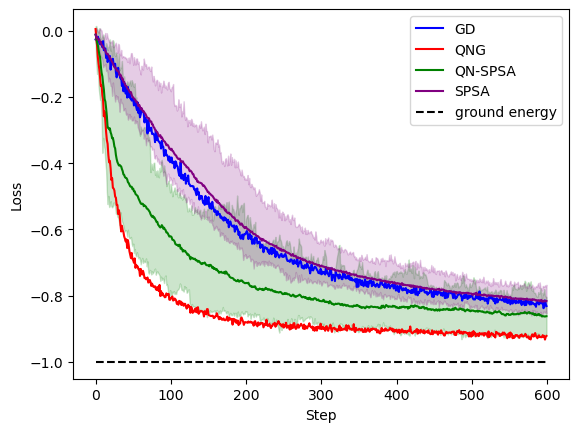
\includegraphics[width=0.7\linewidth]{imagenes/comparacionAlgoritmosOptimizacion.png}
  \caption{Comparativa de los algoritmos de optimización \gls{gd}, \gls{spsa}, \gls{qng} y \gls{qn-spsa} en términos de convergencia y coste computacional. Fuente: \cite{duan_qnspsa_pennylane_2022}.}
  \label{fig:comparacion_optimizadores}
\end{figure}

Como se puede apreciar, en esta comparativa el que obtiene mejores resultados en número de iteraciones es \gls{qng}. Sin embargo, esta representación no contempla el tiempo de ejecución. Como se comentó anteriormente, el optimizador \gls{qng} requiere el cálculo exacto del tensor métrico en cada iteración, lo que demanda un número de mediciones que escala con el cuadrado de los parámetros ($\mathcal{O}(d^2)$) y lo hace computacionalmente inviable a gran escala. Con esto se demuestra que el optimizador \gls{qn-spsa} es el que mejor resultado ofrece de manera equilibrada: logra una pérdida (\textit{loss}) baja con un coste de medición constante ($\mathcal{O}(1)$) y un tiempo de ejecución significativamente menor, consolidándose como una opción altamente escalable.

\subsection{Inicialización guiada de parámetros (\textit{Educated Guess})}
\label{subsec:educated_guess}

La segunda propuesta de mejora aborda la dependencia del entrenamiento respecto a la inicialización de los parámetros del circuito. El artículo de referencia \cite{ohno_qword2vec_2025} inicializa todos estos parámetros a cero, lo que sitúa al optimizador en un punto de partida arbitrario del espacio de parámetros sin ninguna garantía de proximidad a una región favorable.

En este trabajo se introduce una estrategia de inicialización informada, denominada \textit{educated guess}, que evalúa un conjunto de puntos de inicio aleatorios antes de comenzar la optimización y selecciona aquel con menor pérdida. En concreto, se generan 10 configuraciones iniciales de parámetros muestreadas aleatoriamente, se evalúa la función de pérdida del circuito para cada una de ellas, y se adopta como punto de partida la configuración que produce el menor valor de pérdida. De este modo, el optimizador comienza su búsqueda desde una región ya orientada hacia un mínimo prometedor del espacio de parámetros.

Esta técnica aporta dos ventajas principales. En primer lugar, elimina la necesidad de un paso de aprendizaje agresivo para explorar regiones lejanas del espacio de parámetros, ya que el punto de partida se encuentra en una zona favorable. En segundo lugar, reduce el impacto del ruido inherente a las primeras iteraciones del entrenamiento. Los valores de pérdida de un circuito variacional cuántico sin pesos preentrenados suelen ser muy inestables debido a la alta varianza de las estimaciones obtenidas por el muestreo finito del simulador. Por tanto, partir de una configuración inicial optimizada proporciona una mayor estabilidad y contribuye a una convergencia más robusta.

La combinación de esta inicialización guiada con el optimizador \gls{qn-spsa} descrito en la sección anterior constituye el núcleo de las propuestas de mejora de este trabajo.
